\documentclass[a4paper,10pt]{article}
\newcommand{\path}{../../../mygit/_Latex/}
\input{\path StdPack.tex}
\usepackage{\path cmds}
\graphicspath{{figures/}}

\begin{document}


\title{Simulation of Dynamical Scattering Effect in Macromolecular Electron Diffraction Patterns}
\author{Tarik Drevon, David Waterman, Eugene Krissinel}

\maketitle
\addcontentsline{toc}{section}{Contents}
\tableofcontents

%%%%%%%%%%%%%%%%%%%%%%%%%%%% Begin Document

% \begin{abstract}
% Here
% \end{abstract}


\section{Introduction}
Macromolecular structures have been successfully solved with
Electron diffraction(ED) patterns and standard macromolecular X-ray crystallographic(MX) techniques since 2013~\cite{ShiNanenga2016,ClabbersGrueneAbrahams2017}.
This technique is currently refered to as microED.
In practice, growing good quality macromolecular crystals up to micrometric sizes is often a challenge and even sometimes impossible.
MicroED is therefore a very appealing technique because it enables solving structures from nanocrystals. Another interesting aspect is that ED patterns provide information about the electrostatic potential which is a complementary information to the electron density maps provided by X-ray diffraction patterns. Besides, ED patterns may provide higher resolution than the more popular cryo-EM imaging technique~\cite{Latychevskaia2019}.
However, theoretical works~\cite{GlaeserDowning1993,SubramanianSpence2015} have suggested that dynamical diffraction effects are too prominent for macromolecular crystals larger than a few tens of nanometer to allow the use of standard MX techniques for structure determination.

In this work, simulations of ED patterns are performed with the multislice algorithm(MS)~\cite{CowleyMoodie1957,Ishizuka2004,Kirkland2019} as an
attempt to explain the discrepancies between theory and experiment.

The first section presents the MS algorithm, the second section shows an example for a 2-beam diffraction setup
The third section presents simulates are performed on small molecules such as biotin.


\section{Multislice algorithm}\label{chap:MS}

The multislice approach solves Schrodinger's equation for the incident electron beam assuming its kinetic energy is far greater than the specimen potential. This results in the real space fast electron Schrodinger's equation \cite{Kirkland2019}:
\begin{equation}\label{eq:FESE}
  \frac{\dP\Psi(x,y,z)}{\dP_z} =
    \Big\{\frac{i\lambda}{4\pi}\grad^2_{xy} + i\sigma V(x,y,z)\Big\} \Psi(x,y,z)
\end{equation}
where $\Psi$ is the elctron wavefunction,
$V(x,y,z)$ the specimen potential and
$\sigma=2\pi m_0e\lambda/h^2$($rad/kV\ang$) the interaction parameter, $\lambda$ being the relativistic electron wavelength, $m_0$ the electron rest mass, $e$ the elementary charge and $h$ plank's constant.

A direct integration along the incident beam direction $z$ gives :
\begin{equation}
  \Psi(z+\Delta z) = \Psi(z)
  \exp\left(i\lambda/4\pi\Delta z\grad^2_{xy}\right)
  \exp\left(i\sigma\nu_{\Delta z}(x,y,z)\right)
\end{equation}
where $\nu_{\Delta_z}=\int_z^{z+\Delta z}V(x,y,z^{'})dz^{'}$
is the projected potential.

The exponentiation operator can be approximated as a propagator convolution :
\begin{equation}\label{eq:MS_conv}
  \Psi(x,y;z+\Delta z) = p(x,y;\Delta z)\ast\Big(t(x,y,z)\Psi(x,y;z)\Big)
  +\mathcal O(\Delta z^2\nu_{\Delta z})
\end{equation}
where $t(x,y;z)=e^{i\sigma\nu_{\Delta z}}$ is the transmission function, and $p(x,y;\Delta z)=\frac{1}{i\lambda\Delta z}e^{ik_0\frac{x^2+y^2}{2\Delta z}}$ the Fresnel propagator.

Since convolutions can be very efficiently computed using the Fourier transform convolution theorem, the multislice algorithm is performed in practice as :
\begin{equation}\label{eq:MS_FFT}
  \Psi(x,y;z+\Delta z) \approx FFT^{-1}\Bigg\{
    P(k_x,k_y;\Delta z) FFT\Big(t(x,y;z)\Psi(x,y;z)\Big)
  \Bigg\}
\end{equation}
where $P(k_x,k_y;\Delta z)=e^{-i\pi\lambda\Delta z(k_x^2+k_y^2)}$ is the Fresnel Propagator Fourier transform, $FFT$ and $FFT^{-1}$ being the Fourier transform and its inverse.




\newpage
\section{Application to 2-beam theory}\label{chap:2_beam_theory}
The effect of dynamical diffraction can be demonstrated using the 2-beam configuration problem. In this configuration, 2 beams (a central beam $\bb o$ and a diffracted beam $\bb g$) are at the Bragg condition while all other beams are far from the Bragg condition hence very weakly excited.

In 2 beam theory~\cite{ZuoSpence2016}, the intensity of the non central beam should be :
\begin{equation}\label{eq:I_dyn2}
  I_{dyn-2}(S_g;t,\xi_g) =
    \frac{\sin^2\left(\frac{\pi t}{\xi_g}
    \sqrt{1+S_g^2\xi_g^2}\right)}{1+S_g^2\xi_g^2}
\end{equation}
where $S_g$($\ang^{-1}$) is the excitation error i.e. the distance in reciprocal space between $q=\sin\theta/\lambda$ and the location of Bragg beam $\bb g$.
$t$($\ang$) is the thickness,
$\xi_g=k_0/U_g$ (in $\ang$) is the Pendellosung thickness .
$k_0=1/\lambda$ (in $\ang$) the incident electron wave number ,
$U_g=2me/h^2 v_g$(in $\ang^{-2}$) the structure factor and $v_g$ (in $V$) the electrostaic potential Fourier components of Bragg beam $\bb g$.

In contrast, in the kinematic case :
\begin{equation}\label{eq:I_kin}
  I_{kin}(S_g;t,v_g) = \left(\sigma v_g t\right)^2\
  \frac{\sin^2\left(\pi S_gt\right)}{\pi S_g t}
\end{equation}
where $\sigma v_g=\pi/\xi_g$ so that \eqref{eq:I_kin} is a limit case of \eqref{eq:I_dyn2} for large $\xi_g$ i.e. weak potential.





\subsection{Simulation setup}

For illustrative purposes, a simple 2D monoatomic primitive square lattice of side $a=2\AA$ is simulated with MS.
The crystal is oriented along the $[10 1]$ axis. Due to periodic boundary conditions imposed by the MS algorithm, this requires simulating a $10\times10$ super cell as shown in the electrostatic potential map figure~\ref{fig:2_beam_V}.
The accelerated voltage is voluntary chosen at $E=3.75keV$ to allow for  Ewald sphere curvature. The configuration of the Ewald sphere is shown figure~\ref{fig:2_beam_E} where the blue dots correspond to the original reciprocal lattice rotated by $0.1rad$ from the zone axis $[1 0]$ and the black dots correspond to the reciprocal lattice of the $10\times10$ super cell setup. The blue dots indicate miller indices $h=0,1,2$ where $h=0$ and $h=2$ are at the Bragg condition.

\begin{figure}[h!]
	\begin{subfigure}{0.45\textwidth}
		\centering
		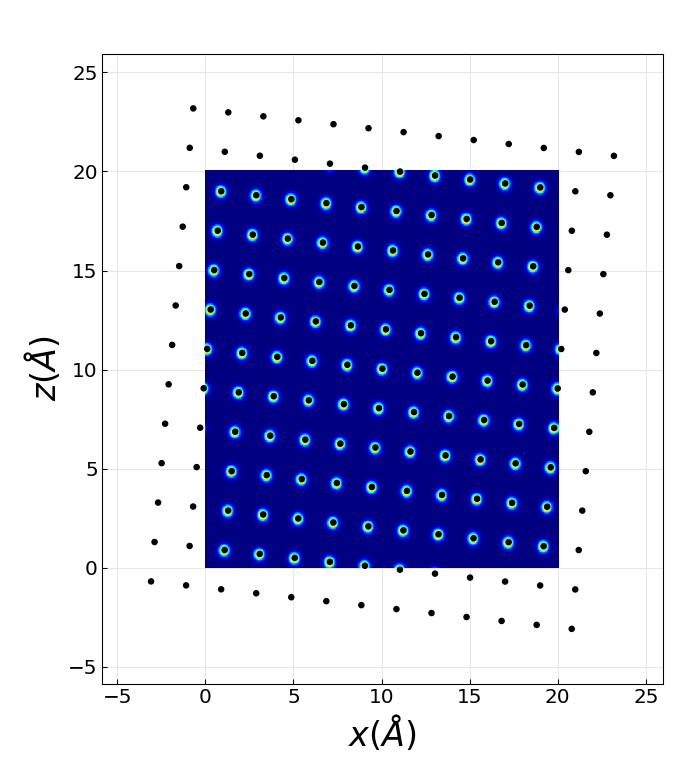
\includegraphics[width=\textwidth]{2_beam_fv.png}
		\caption{}\label{fig:2_beam_V}
	\end{subfigure}
	\begin{subfigure}{0.45\textwidth}
		\centering
    \def\svgwidth{\columnwidth}
		\input{figures/2_beam_E.pdf_tex}
		\caption{}\label{fig:2_beam_E}
	\end{subfigure}

	\caption[2-beam configuration]{
		\ref{fig:2_beam_V} Electrostatic potential map for the $10\times10$ super cell (Blue area).
		\ref{fig:2_beam_E} Ewald circle configuration with $E=3.75keV$. Original reciprocal lattice (blue dots) rotated by $0.1rad$ from the zone axis $[1 0]$ and reciprocal lattice of the $10x10$ super cell (black dots).
	}\label{fig:2_beam_config}
\end{figure}


The diffraction pattern is shown~\ref{fig:2_beam_P} and the major beam intensities as a function of crystal thickness are shown in figure~\ref{fig:2_beam_B} where clear oscillations appear for the excited beam pair $h=0,2$.

\begin{figure}[h!]
  \begin{subfigure}{0.45\textwidth}
    \centering
    \def\svgwidth{\columnwidth}
    \input{figures/2_beam_Iq.pdf_tex}
    \caption{}\label{fig:2_beam_P}
  \end{subfigure}
  \begin{subfigure}{0.45\textwidth}
    \centering
    \def\svgwidth{\columnwidth}
    \input{figures/2_beam_Iz.pdf_tex}
    \caption{}\label{fig:2_beam_B}
  \end{subfigure}
\caption[2-beam diffraction]{
  \ref{fig:2_beam_P} 2 beam diffraction pattern.
  \ref{fig:2_beam_B} Beam intensity as function of sample thickness.
}\label{fig:2_beam_diff}
\end{figure}



\subsection{Extinction distance}

The same simulation is run for different potential strengths corresponding to different atoms. A very weak potential can also be used to mimic the X-ray diffraction pattern.

In figure~\ref{fig:2_beam_I1} the Beam $g_1$ is not at the exact Bragg condition and its intensity with crystal thickness is mostly due to Ewald sphere curvature. Indeed, the oscillation period is independent of the potential strength and mostly depends on excitation error.

On figure~\ref{fig:2_beam_I2}, on the other hand, the beam for $h=2$ is at the Bragg condition and its extinction distance is sensitive to the strength of the potential.
For this strongly excited beam, dynamical diffraction is present at all potential strengths but the kinematic regime is extended to larger crystal thickness at weaker potential.

\begin{figure}[h!]
	\begin{subfigure}{\textwidth}
		\centering
		\begin{subfigure}{0.3\textwidth}
			\centering
      \def\svgwidth{\columnwidth}
			\input{figures/2_beam_I1.pdf_tex}
			\caption{}\label{fig:2_beam_I1}
		\end{subfigure}
		\begin{subfigure}{0.3\textwidth}
			\centering
      \def\svgwidth{\columnwidth}
			\input{figures/2_beam_I2.pdf_tex}
			\caption{}\label{fig:2_beam_I2}
		\end{subfigure}
		\begin{subfigure}{0.3\textwidth}
			\centering
      \def\svgwidth{\columnwidth}
			\input{figures/2_beam_xi.pdf_tex}
			\caption{}\label{fig:2_beam_xi}
		\end{subfigure}
  \end{subfigure}
	\caption[2-beam extinction]{
    Evolution of the
		\ref{fig:2_beam_I1} In
	}\label{fig:2_beam_zeta}
\end{figure}


\subsection{Rocking curve}
Rocking curves are simulated by running simulations varying the beam tilt angles from 0 to 0.08 degrees.

The actual exact Bragg condition is satisfied for the $\theta_c=0.0385^{\circ}$.
At this tilt angle, the Pendullosung thickness can be measured on the $I_b(z)$ giving $\zeta_g=293nm$.
The analytical approach would give $\zeta_g=\pi/\sigma f_v(\theta_i,Z_a)$.

The rocking curves around $\theta_c$ are characteristic of 2-beam theory and shown for $z_{thick}=\left(0.25,0.5,0.75,1,1.25,1.5\right)\zeta_g$.

\begin{figure}[h!]
	\begin{subfigure}{\textwidth}
		\centering
		\begin{subfigure}{0.45\textwidth}
			\centering
      \def\svgwidth{\columnwidth}
			\input{figures/2_beam_rocking.pdf_tex}
			\caption{}\label{fig:2_beam_rocking}
		\end{subfigure}
		\begin{subfigure}{0.45\textwidth}
			\centering
      \def\svgwidth{\columnwidth}
			\input{figures/2_beam_Itheta_c.pdf_tex}
			\caption{}\label{fig:2_beam_Itheta_c}
		\end{subfigure}
  \end{subfigure}
	\caption[2-beam extinction]{
		\ref{fig:2_beam_rocking} Rocking curves obtained at sample thickness $z_{thick}=\left(0.25,0.5,0.75,1,1.25,1.5\right)\zeta_g$.
		\ref{fig:2_beam_Itheta_c} Beam intensities for $h=0,1,2$ as function of sample thickness for crystal rotation $0.1+\theta_c$ where beam $h=2$ is at the exact Bragg condition.
	}\label{fig:2_beam_rocking}
\end{figure}





%%%%%%%%%%%%%%%%%%%%%%%%%%%%%%%%%%%%%%%%%%%%%%%%%%%%%%%%%%%%%%%%%%%%%%%%
% NEAR BRAGG
%%%%%%%%%%%%%%%%%%%%%%%%%%%%%%%%%%%%%%%%%%%%%%%%%%%%%%%%%%%%%%%%%%%%%%%%
\newpage
\section{Near Bragg : Hydrid particle-wave approach}
An alternative approach to the multislice algorithm consists in solving~\eqref{eq:FESE} approximately using an extension of the kinematic theory to multiple scattering.

Each atom scatter the incident electron beam according to its electron-atom scattering cross section. The path length of the incident beam is computed and interference at computed at selected pixels on a detector some distance away from the sample.

\subsection{Scattering by individual atoms}
The first order approximation yields the kinematic theory of diffraction also known as first Born approximation. It is a perturbation treatment often used to allow for an analytical treatment. The incident state $\phi$ is used in place of $\Psi$ in the right hand side so that the scattering equation can readily be solved as :
\begin{equation}
    \Psi(\bb r)=e^{ikz} + f(\theta)\frac{e^{i\bb k\cdot\bb r}}{|\bb r|}
\end{equation}
where :
\begin{equation}
    f(\theta) = -\frac{2me}{h^2}\int d^3re^{i\bb q\cdot\bb r}V(r)
~~\mbox{,     }~~
    \frac{d\sigma}{d\Omega} = |f(\theta)|^2
\end{equation}

where $f(\theta)$ is the scattering amplitude, i.e. the Fourier transform of the electrostatic potential.
In the first Born approximation the far field diffraction pattern is proportional to the square of the scattering amplitude which is known as the differential cross section $\sigma$.


\subsection{Kinematic calculation}
The contribution of atom $j$ to the intensity value at detector pixel $i$ is given by the interference term $\exp(ik_0 R_{ij})/R_{ij}$ where  $R_{ij}$ is the path length from atom $j$ to pixel $i$.
It is written with increasing level of approximations as :
\begin{eqnarray}
R_{ij}
      &\underset{Greens}{=}& \sqrt{\left(x-x_0\right)^2+\left(z-z_0\right)^2} \\
       &\underset{Fresnel}{\approx}&     \left(z_0-z\right) + \frac{\left(x-x_0\right)^2}{2\left(z_0-z\right)} \\
       &\underset{Fraunhofer}{\approx}&  \left(z_0-z\right) + \frac{x_0^2}{2\left(z_0-z\right)} - \frac{xx_0}{\left(z_0-z\right)}  \\
\end{eqnarray}

For planar illumination, the path length from the source the to atom $j$ is $z$ and must be added to the path length in the expo


\begin{figure}[h!]
	\begin{subfigure}{\textwidth}
		\centering
		\begin{subfigure}{0.45\textwidth}
			\centering
      \def\svgwidth{\columnwidth}
			\input{figures/2_beam_rocking.pdf_tex}
			\caption{}\label{fig:2_beam_rocking}
		\end{subfigure}
		\begin{subfigure}{0.45\textwidth}
			\centering
      \def\svgwidth{\columnwidth}
			\input{figures/2_beam_Itheta_c.pdf_tex}
			\caption{}\label{fig:2_beam_Itheta_c}
		\end{subfigure}
  \end{subfigure}
	\caption[2-beam extinction]{
		\ref{fig:2_beam_rocking} Rocking curves obtained at sample thickness $z_{thick}=\left(0.25,0.5,0.75,1,1.25,1.5\right)\zeta_g$.
		\ref{fig:2_beam_Itheta_c} Beam intensities for $h=0,1,2$ as function of sample thickness for crystal rotation $0.1+\theta_c$ where beam $h=2$ is at the exact Bragg condition.
	}\label{fig:2_beam_rocking}
\end{figure}


% comparison | error
% ---------- | ---------
% [<img src="/projects/nearBragg/figures/path_length.svg" width="350" /> ](/projects/nearBragg/figures/path_length.svg) | [<img src="/projects/nearBragg/figures/path_length_diff.svg" width="350" /> ](/projects/nearBragg/figures/path_length_diff.svg)



% The probabilities of an electron to undergo $m$ elastic collisions and $n$ inelastic collisions of mean free path $l_i$ after going through a specimen of length $z$ follows the Poisson distribution :
% \begin{equation}
%   P_{mn}(z) =
%     \frac{1}{m!}\left(\frac{z}{l_e}\right)^me^{-z/l_e}
%     \frac{1}{n!}\left(\frac{z}{l_i}\right)^ne^{-z/l_i}
% \end{equation}
% where
%
% - $l_e=1/\sigma_e\rho$ is the average elastic collision mean free path, $\sigma_e=|f^{(e)}_a|^2$ being the interaction cross section and $f^{(e)}_a$ the atomic elastic scattering factor.
% - $l_i=1/\sigma_i\rho$ is the average inelastic collision mean free path.
% - $\rho$ is the number of atoms per volume area.
%
% [Latychevskaiaabrahams2019](/readings/papers/#latychevskaiaabrahams2019) followed a similar approach where the order of the collisions is considered to determine which sequence of events contribute to Bragg spots. A simplification of her equations considering only 0,1 and more than 1 elastic collisions reads :
% \begin{eqnarray}
%   P_{coh}(z+dz) &=& (1-P_e(dz))P_{coh}(z) \\
%   P_{kin}(z+dz) &=& (1-P_e(dz))P_{kin}+P_e(dz)P_{coh}(z) \\
%   P_{dyn}(z+dz) &=& P_{dyn}(z) + P_e(z)P_{kin} \\
% \end{eqnarray}
%
% which analytical solutions are the Poisson distribution above. The program [nearBragg](/projects/nearBragg) should follow this statistics. Taking for protein $\rho=106$ atoms per $nm^3$ and $\sigma_e=0.001-0.005A^2$ which covers beam energies $E=100-1000keV$ and protein average scattering powers give mean free paths ranging $l_e=200-1000nm$.
%
% small $\sigma_e$ | medium $\sigma_e$ | large $\sigma_e$
% ---------------- |------------------ | ----------------
% [<img src="/projects/nearBragg/figures/Pcoh_kin_dyn0.svg" width="350" /> ](/projects/nearBragg/figures/Pcoh_kin_dyn0.svg) | [<img src="/projects/nearBragg/figures/Pcoh_kin_dyn1.svg" width="350" /> ](/projects/nearBragg/figures/Pcoh_kin_dyn1.svg) | [<img src="/projects/nearBragg/figures/Pcoh_kin_dyn2.svg" width="350" /> ](/projects/nearBragg/figures/Pcoh_kin_dyn2.svg)



%%%%%%%%%%%%%%%%%%%%%%%%%%%% End Document
\newpage
% \thispagestyle{empty}
% \mbox{}
% \newpage
\bibliographystyle{ieeetr}
\bibliography{\path library}
\addcontentsline{toc}{section}{References}
\end{document}
